\documentclass[12pt]{article}
\usepackage{amsmath}
\usepackage{graphicx}
\usepackage{float}
\begin{document}
\title{Coffee Cooling Challenge \#2}
\author{Daniel Huantes}
\twocolumn
\maketitle
\section{Introduction}
For this weeks challenge we used numerical methods in order to solve a first order seperable differential equation. The specific method we used was odeint, a function found in scipy's integrate module. The problem we dealt with was using the differential form of Newtons law of cooling 
\begin{equation}
\frac{\mathrm{d} T(t)}{\mathrm{d} t} = -r (T(t) - T_{env})
\end{equation}
with T(t) being the temperature of the coffee in our cup as a function of time, T$_{env}$ being the temperature of the room the cup was in, and r to be a physical constant defined as 
\begin{equation}
r = \frac{hA}{mc}
\end{equation}
We assumed that the room was large enough that any heat transferred from the cup to the environment through cooling would have a negligible effect on the temperature of the room. Our heat loss was modeled entirely through the area of the cup that was exposed to the air, and we assumed a container holding the coffee that would not lose any heat to the sides to the mug wall in order to simplify our problem.
\section{Discussion}
First, we set up our imports, numpy, scipy, matplotlib and our odeint function. Next we set up global variables representing the given quantities that were provided in the challenge document and videos. The global variables T\_env and T0, representing $T_{env}$ and $T(0)$ respectively, are now iniialized to a temperature in $^o$Farenheight. The expressions following their initialization converts them to $^o$Celcius, in order to be compatible with the units included. After this, I defined my function coolingLaw with two parameters, T and t, and had it return the temperature encapsulated in a numpy array. The function expects T to be a list-like argument, as it used it's zeroth index for T(t). The r constant and T$_{env}$ from Newton's law of cooling are referenced from the previously set up global variables. Odeint expects the method representing the differential to take two inputs, although there is an option to include additional arguments in a tuple at the end of the arguments of odeint to pass any further arguments to the function. Odeint's two other arguments other than the function it solves are the temperatures and times. Both were passed as numpy arrays, times being a list of linearly spaced points from 0 to 3600, representing our domain of interesti in seconds, 1 hour, and a list containing one member, the initial temperature of our coffee. We take the zeroth column of odeint's result and place it into a variable called T. Finally, I plotted T against times, using a vector operation inside of the plot call to convert times from seconds to minutes and another to convert our temperatures from $^o$C to $^o$F.
\section{Code}
\begin{figure}[H]
  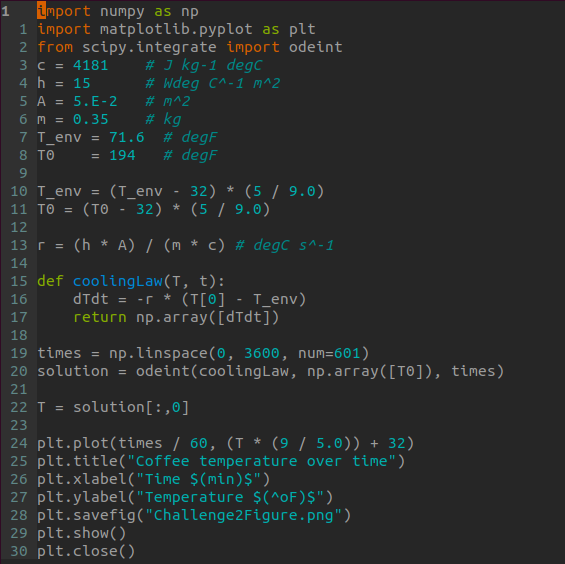
\includegraphics[width=\linewidth]{CodeSnippetCC2.png}
  \caption{My Beautiful Code!}
  \label{fig:mBC}
\end{figure}
\section{Results}
\begin{figure}[H]
  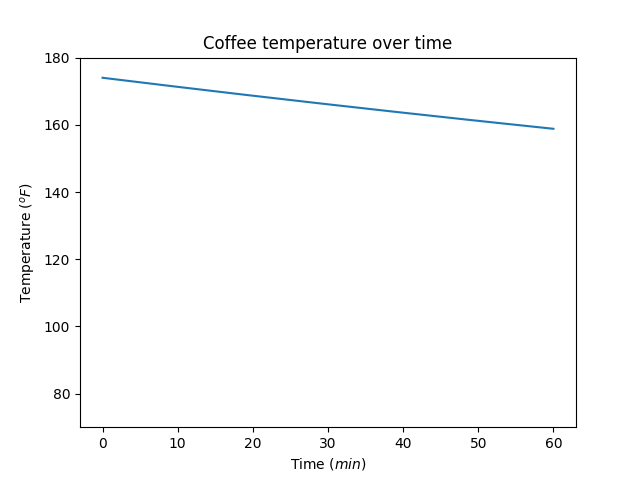
\includegraphics[width=\linewidth]{Challenge2Figure.png}
  \caption{Plot generated from my code}
  \label{fig:plt1}
\end{figure}
The plots shows that as the difference in temperature between the coffee and the surroundings decrease, the rate at which the coffee cools decreases as well, which is consistent with our formula. We can be satisfied that at least under the assumptions we made, that we have successfully used numerical tools in order to solve a differential equation representing the cooling of a coffee cup.
\section{Conclusion}
We can tell that numerical methods to solve differentials are an extremely useful tool, because although the analytical solution to this specific function is fairly easily found, it does save us as programmers some work, as well as give us a tool to use in the future for more differentials. In further work, I plan to model thetemperatures of both the liquid inside the coffee and the cup in which it is held, as well as introducing ideas like variable volume of coffee.
\end{document}

